\documentclass[11pt]{article}

\usepackage[T1]{fontenc}
\usepackage{lmodern}

% Math + symbols
\usepackage{amsmath,amssymb,amsthm,mathtools}
\usepackage{microtype}

% Figures + tables
\usepackage{graphicx}
\usepackage{booktabs}
\usepackage{array}
\usepackage{subcaption}
\usepackage{float}

% Colors
\usepackage{xcolor}

% Page styling
\usepackage{fancyhdr}
\usepackage[margin=1in]{geometry}

% Links
\usepackage{hyperref}
\hypersetup{
  colorlinks=true,
  linkcolor=blue!70!black,
  citecolor=green!50!black,
  urlcolor=blue!80!black,
  bookmarksnumbered=true,
  pdfauthor={Ioannis Tsiokos},
  pdftitle={Six Birds for Navier--Stokes: A Mechanized No-Zeno Scaffold}
}

% References
\usepackage{cleveref}
\crefname{section}{section}{sections}
\crefname{table}{table}{tables}
\crefname{figure}{figure}{figures}

% Bibliography
\usepackage[numbers]{natbib}
\usepackage{orcidlink}

% Local macros
% Notation macros (minimal to start)

\newcommand{\R}{\mathbb{R}}
\newcommand{\N}{\mathbb{N}}
\newcommand{\T}{\mathbb{T}}

\newcommand{\ip}[2]{\left\langle #1, #2 \right\rangle}
\newcommand{\norm}[1]{\left\| #1 \right\|}

\newcommand{\uLtwo}{\norm{u}_{L^2}}
\newcommand{\w}{\omega}

% Theorem environments
\newtheorem{theorem}{Theorem}
\newtheorem{lemma}{Lemma}
\newtheorem{definition}{Definition}
\newtheorem{remark}{Remark}

% Allow line breaks at underscores in \nolinkurl (for long identifiers/paths)
\makeatletter
\g@addto@macro\UrlBreaks{\do\_}
\makeatother

% Draft helpers
\newcommand{\todo}[1]{\textcolor{red}{[TODO: #1]}}


% Prevent widows and orphans
\widowpenalty=10000
\clubpenalty=10000
\raggedbottom

\title{Six Birds for Navier--Stokes: A Mechanized No-Zeno Scaffold}
\author{Ioannis Tsiokos\,\orcidlink{0009-0009-7659-5964}}
\date{15 February 2026}

\newcommand{\printaffiliation}{%
  \begin{center}\small \end{center}%
}

\fancypagestyle{firstpage}{%
  \fancyhf{}
  \fancyfoot[C]{\scriptsize Automorph Inc., Wilmington, DE, USA \quad \texttt{ioannis@automorph.io} \quad DOI: TBD \quad \textcopyright\ 2026 \quad CC-BY 4.0 \quad Preprint --- not peer reviewed.}
  \renewcommand{\headrulewidth}{0pt}
  \renewcommand{\footrulewidth}{0pt}
}

\begin{document}
\maketitle
\thispagestyle{firstpage}
\printaffiliation

\begin{abstract}
Energy estimates for 3D incompressible Navier--Stokes control $L^2$ norms but do not prevent
highly localized gradient peaks, which is why global regularity is typically reduced to
``peak-channel'' criteria (e.g.\ Beale--Kato--Majda \citep{bkm_1984}).
We develop a multiscale \emph{decision scaffold}, inspired by the Six-Primitives/Six-Birds framework,
that separates (i) system-agnostic inequality logic, (ii) Navier--Stokes-facing hinge assumptions,
and (iii) numerical diagnostics.

Operationally, we (A) mechanize in Lean a No-Zeno engine: refinement events are encoded by crossing
times, and Zeno cascades are ruled out under work/capacity/divergence hypotheses; (B) mechanize a
route-stability $\Rightarrow$ polynomial-capacity lemma; and (C) mechanize a discrete no-go theorem:
if the feasible interface inputs at a scale admit highly localized tests, then any uniform ICAP-style
capacity certificate forces a pointwise positive-gain bound---the discrete analogue of a peak/strain
control in the PDE interpretation.
Motivated by this obstruction, we propose an \emph{SBT-legal} variant in which feasibility excludes
strong localization, and we operationalize legality as a reproducible certificate based on
per-shell anti-localization and channel diagnostics.
In numerical demos, typical smooth random seeds pass the certificate with $\max_j \kappa_j=O(1)$,
while intentionally localized shell wavepackets fail immediately (e.g.\ $\max_j\kappa_j\sim 10^2$).

These results clarify exactly where a Clay-style proof would require a genuinely new Navier--Stokes
inequality (a provable channelization/delocalization-to-anti-localization hinge) and provide a
reproducible workflow for testing such hypotheses.
We do not claim a proof of Clay regularity, nor do we prove that the legality certificate is preserved
under the classical Navier--Stokes flow; PDE-facing implications are stated explicitly as OPEN
assumptions.
\end{abstract}

\noindent\textbf{keywords:} Navier--Stokes; multiscale scaffold; No-Zeno engine; route capacity; SPT-legality; peak-channel regularity; Six Birds framework


\section{Introduction}

The Clay Millennium problem for 3D incompressible Navier--Stokes asks whether smooth initial data always generate globally smooth solutions, or whether a finite-time singularity (``blow-up'') can occur. A central reason the problem resists purely energy-based methods is that energy can remain bounded while gradients (or vorticity stretching) form intense, localized peaks. Classical conditional criteria formalize this (e.g.\ Beale--Kato--Majda type peak-channel control): if a certain ``peak channel'' stays integrable in time (e.g.\ a supremum norm controlling vortex stretching), then blow-up cannot occur \citep{bkm_1984}. The open difficulty is to show that such peak control must hold automatically for all smooth initial data.

This paper does \emph{not} claim a solution to the Clay problem. Instead, it builds a sharp, reproducible \emph{decision scaffold} for a multiscale approach inspired by the Six Birds framework \citep{tsiokos_2026_18365949}. The core idea is to treat scale-elimination not as a modeling choice but as a canonical \emph{packaging} operation: the eliminated degrees of freedom become a causal ``bridge object'' acting on the retained variables through an interface, and the overall dynamics are constrained by an \emph{accounting} law. In Six Birds terms, we rely on six recurring structural moves:
(i) rewrite/coordinate change, (ii) feasibility/gating constraints, (iii) route dependence of reductions, (iv) sectorization/quantization of interaction channels, (v) packaging of eliminated structure into an effective object, and (vi) accounting (passivity-like) inequalities \citep{tsiokos_2026_18365949}. Our repo makes this concrete for Navier--Stokes by defining canonical multiscale objects (dyadic shells, frontier scales, and packaged subgrid operators) and then asking which primitive-shaped lemmas would be sufficient to rule out ``Zeno'' cascades to infinite depth.

\paragraph{What is mechanized vs.\ what is evidence.}
We separate three layers of claims:
\begin{itemize}
\item \textbf{MECH (Lean):} We mechanize the pure inequality logic used by the No-Zeno engine: summability implies no finite upper bound on crossing times; work/capacity inequalities imply increment lower bounds; and route-stability inequalities imply polynomial capacity growth. These are system-agnostic and proved in Lean in this repository.
\item \textbf{NUMERIC (Python):} We provide diagnostic computations for Navier--Stokes and toy models (dyadic ladders, route-capacity extraction, anti-localization metrics, and channel diagnostics). These are reproducible from a manifest and produce deterministic metadata; they are evidence, not proofs.
\item \textbf{OPEN (assumptions):} The Navier--Stokes-facing hinge lemmas that would be required for a Clay claim are stated explicitly as open assumptions, with no ambiguity about what remains unproved.
\end{itemize}

\paragraph{The core insight: where Clay collapses in this scaffold.}
Our initial goal was to certify a ``No-Zeno'' condition: that the multiscale frontier cannot climb to arbitrarily fine scales in finite time. A natural route is to bound a positive-work ``capacity'' of the packaged subgrid bridge and then show a divergence condition that forces crossing-time sums to diverge. However, a discrete no-go theorem (mechanized in an appropriate finite-dimensional form) shows a fundamental obstruction: if the feasible interface inputs at scale $j$ remain rich enough to approximate localized wavepackets, then any \emph{uniform} ICAP-style certificate for the bridge implies a pointwise bound on a positive-gain functional---a peak/strain bound in the PDE interpretation. In other words, unless feasibility \emph{excludes localization}, the ``capacity'' route is not easier than classical peak-channel criteria; it implicitly contains them.

\paragraph{What we do instead: an SBT-legal Navier--Stokes variant.}
Rather than chasing Clay as stated, we formalize and study a sharpened program: define an operational notion of \emph{SBT-legal} initial data that forbids extreme localization at dyadic scales, motivated by the channelization/anti-localization hinge required to escape the wavepacket obstruction. Concretely, we implement a certificate that measures anti-localization metrics per shell (normalized concentration factors, burst ratios, and effective channel counts), and we show (numerically) that typical smooth random seeds pass while intentionally constructed localized shell wavepackets fail immediately. This does not prove global regularity for all smooth data; it clarifies a precise, testable boundary between ``legal'' and ``illegal'' regimes for the Six Birds program.

\paragraph{Contributions.}
The repository accompanying this paper provides:
\begin{itemize}
\item a mechanized No-Zeno algebra chain (Lean) and a mechanized route-capacity polynomial-growth theorem;
\item mechanized discrete lemmas capturing (i) anti-localization from delocalized finite channels and (ii) the ICAP$\Rightarrow$peak-control no-go under localization-rich feasibility;
\item a manifest-driven, deterministic figure generator producing all paper artifacts and metadata;
\item a concrete SBT-legality certificate and an explicit illegal-vs-legal initial condition demo.
\end{itemize}

\paragraph{Reading guide.}
Section~2 recalls the Six Birds framework and maps it to the Navier--Stokes multiscale objects used here. Sections~3--4 present the No-Zeno and route-capacity logic (Lean-mechanized). Section~5 states the no-go obstruction and its discrete mechanization. Sections~6--7 define the SBT-legal certificate and present the reproducible diagnostics and figures. We conclude with limitations and open questions in Section~8.

\section{Six Birds recap and mapping to Navier--Stokes objects}
\label{sec:six_primitives_mapping}

This section gives a compact, self-contained recap of the Six Birds framework and fixes the specific mathematical objects used throughout the rest of the paper. Our presentation is intentionally operational: we only introduce the parts of the framework that are used in the No-Zeno scaffold and in the ``SBT-legal'' diagnostics. For the broader theory and motivation we refer to the original Six Birds paper \citep{tsiokos_2026_18365949}. For standard Navier--Stokes background see, e.g., \citet{temam_ns} or \citet{majda_bertozzi_vif}.

\subsection{Six Birds as an interface calculus (one paragraph each)}
\label{sec:six_primitives_recap}

We use the Six Birds as a \emph{structured way to talk about multiscale elimination} without committing to a particular closure ansatz. In the language of \citet{tsiokos_2026_18365949}, each ``primitive'' is a recurring move that appears across physical and abstract systems; here we specialize them to a dyadic-scale analysis of incompressible Navier--Stokes.

\paragraph{P1: Rewrite (change of description).}
We choose a representation in which scale is explicit. In this repository that is a Littlewood--Paley decomposition into dyadic shells \citep{bahouri2011fourier}:
\[
u(t,x)=\sum_{j\ge 0} u_j(t,x),\qquad u_j:=\Delta_j u,\qquad u_{\le j}:=G_j u.
\]
This is not a modeling assumption; it is a change of coordinates that turns ``fine scales'' into explicit indices.

\paragraph{P2: Feasibility / gating (what inputs are allowed).}
Not every formal ``port signal'' should be regarded as physically admissible. We formalize admissibility in two places:
(i) in the definition of the packaged bridge, where only low-pass histories for which a coupled high-pass IVP is well-posed are allowed, and
(ii) in the paper's ``SBT-legality certificate,'' which empirically tests whether a given initial condition is \emph{anti-localized} across shells (ruling out wavepacket-like concentration).

\paragraph{P3: Route dependence (noncommuting reductions).}
Eliminating degrees of freedom in different orders can yield different effective descriptions. The paper isolates a route-mismatch quantity and proves an abstract Lean theorem showing that \emph{summable} mismatch plus tame local inflation yields \emph{polynomial} growth of effective capacity. This is the only place the framework can plausibly add leverage beyond classical one-shot estimates.

\paragraph{P4: Sectorization / quantization (finite channel structure).}
Interactions are not arbitrary; they often decompose into a bounded number of ``channels'' (sectors/atoms). In this repo we treat channelization as a measurable property: we estimate an effective channel count $m_j$ per shell (via pooled SVD/PCA diagnostics) and measure delocalization of the learned channels. The paper also mechanizes a finite-dimensional lemma showing that a finite set of delocalized channels forces anti-localization bounds for feasible inputs.

\paragraph{P5: Packaging (turn eliminated structure into an effective object).}
Packaging converts ``everything above scale $j$'' into a causal, memoryful \emph{bridge object} acting on the retained variables through an interface. For Navier--Stokes we define a canonical packaged bridge $Z_j$ by coupling a low-pass history to a high-pass IVP and reading off the induced subgrid influence on shell $j$. This is a definition, not a fit: $Z_j$ is not assumed linear or time-invariant.

\paragraph{P6: Accounting (passivity-like inequalities).}
Accounting is the constraint that the packaged bridge is not arbitrary: it must respect an energy/work ledger in the spirit of dissipativity/passivity formulations \citep{willems1972dissipative1}. In the No-Zeno engine we use a positive-work functional $W_j^+$ as the currency, and (optionally) a storage functional $S_j$ to define a ``frontier'' process whose advance requires fresh work.

\subsection{Canonical Navier--Stokes objects fixed in this repo}
\label{sec:ns_object_mapping}

We now list the NS objects that serve as the paper's \emph{single source of truth}. The goal is that later sections can refer back here without ambiguity.

\paragraph{Dyadic shells and ports.}
On $\mathbb{T}^3$, let $\Delta_j$ be the standard Littlewood--Paley shell operators and $G_j$ the low-pass operator. Define
\[
u_j:=\Delta_j u,\qquad u_{\le j}:=G_j u,\qquad U_j:=\mathrm{Ran}(\Delta_j)\cap L^2_\sigma(\mathbb{T}^3).
\]
The \emph{port input at scale $j$} is $u_j(t)\in U_j$.

\paragraph{Environment influence and closure term.}
Write the nonlinear term as $\mathrm{NL}(u):=\mathcal{P}\nabla\cdot(u\otimes u)$ where $\mathcal{P}$ is the Leray projector. The low-pass evolution sees an ``environment influence'' consisting of the nonlinear interactions involving $u_{>j}$. The repository records the canonical algebraic identities in the blow-up docs and uses them for diagnostic computations (not as a closure model).

\paragraph{Packaged bridge object $Z_j$.}
Fix $T>0$ and $s>5/2$. For a low-pass history $v$ with $G_j v=v$ on $[0,T]$, solve the coupled high-pass IVP for $w$ driven by $v$ (when well-posed), and define
\[
Z_j[v](t)\in U_j
\quad\text{as the induced shell-$j$ output extracted from the canonical subgrid term.}
\]
The formal, fully specified definition (spaces + causality + coupling) is in
\nolinkurl{docs/fluids/blowup/ns_bridge_object.md}.
We emphasize: $Z_j$ is not assumed linear, time-invariant, or computable; it is a mathematically meaningful object attached to the NS evolution.

\paragraph{Power and positive-work currency.}
Given a port input $u_j(t)$ and a bridge output $y_j(t):=Z_j[u_{\le j}](t)$ (or a suitable proxy when discussing abstract inequalities), define the instantaneous power and its positive part:
\[
p_j(t):=\langle u_j(t),y_j(t)\rangle_{L^2},\qquad p_j^+(t):=\max(p_j(t),0),
\]
and the positive work on a window $[s,t]$:
\[
W_j^+[s,t]:=\int_s^t p_j^+(\tau)\,d\tau.
\]
This is the ``accounting currency'' used in the No-Zeno scaffold.

\paragraph{Capacity and the No-Zeno engine (abstract, mechanized).}
The abstract engine uses inequalities of the form
\[
W_j^+[s,t]\le \Lambda(j)\int_s^t \|u_j(\tau)\|_{L^2}^2\,d\tau,
\]
together with a work-quantum condition (frontier advance forces $W_j^+\ge \theta$) and a divergence condition on $\sum 1/\Lambda(j)$.
All purely algebraic steps of this chain are mechanized in Lean (see \texttt{formal/Fluids/*.lean}) and summarized in
\texttt{docs/fluids/blowup/clay\_chain\_scaffold.md}.

\paragraph{Route mismatch and capacity growth (abstract, mechanized; NS evidence only).}
The repository mechanizes an abstract theorem: if a depth-indexed capacity sequence obeys a tame multiplicative inflation bound with summable additive mismatch, then capacity growth is polynomial in depth (not exponential). This is a general statement about reductions/packaging routes; connecting it to NS is currently supported by diagnostics (not a proof), and the exact status is recorded in \texttt{docs/fluids/blowup/theorem\_inventory\_blowup.md}.

\section{The No-Zeno engine (mechanized algebra)}\label{sec:no-zeno-engine}

This section isolates the \emph{pure inequality logic} behind our ``No-Zeno'' decision engine.
Nothing here is specific to Navier--Stokes: the same argument applies to \emph{any} multiscale
process whose refinement events admit (i) an increment lower bound and (ii) a divergence check.
All PDE content enters later only through attempting to justify the hypotheses (WORK/CAP/DIV).

\paragraph{Mechanization boundary.}
All results in this section are mechanized in Lean in a discrete setting:
crossing times are sequences $t:\N\to\R$ and hypotheses are stated using finite sums over $\N$.
Continuous-time integral inequalities are used later only as motivational analogues and are not
formalized in this paper.

\subsection{Crossing times and the Zeno condition}

Let $t:\N\to\R$ be an increasing sequence of \emph{crossing times}, where $t(n)$ is interpreted as
the first time a multiscale ``frontier'' reaches level $n$ (e.g.\ a shell index threshold).
Define increments
\[
\Delta t_n := t(n+1)-t(n)\qquad (n\in\N).
\]

\begin{definition}[Zeno cascade]\label{def:zeno}
We say a \emph{Zeno cascade} occurs if the crossing times are bounded above:
\[
\exists\,T\in\R\ \ \text{s.t.}\ \ \forall n\in\N,\ t(n)\le T.
\]
Equivalently, $\sup_n t(n)<\infty$, i.e.\ the frontier reaches arbitrarily fine levels in finite time.
\end{definition}

\subsection{Increment lower bounds imply No-Zeno}

The basic mechanism is: if each increment $\Delta t_n$ is bounded below by a nonnegative
quantity whose partial sums are unbounded, then $t(n)$ cannot remain bounded.

\begin{definition}[Increment certificate]\label{def:phi}
Let $\Phi:\N\to\R$ be a nonnegative sequence. We say $\Phi$ is an \emph{increment certificate}
for $t$ if for all $n$,
\[
\Phi(n)\ \le\ t(n+1)-t(n).
\]
\end{definition}

\begin{theorem}[Unbounded partial sums imply no finite upper bound]\label{thm:unbounded-sums-no-zeno}
Assume $\Phi$ is an increment certificate for $t$ and that its partial sums are unbounded:
\[
\forall M\in\R,\ \exists n\in\N\ \text{s.t.}\ M \le \sum_{k=0}^{n-1}\Phi(k).
\]
Then $t$ has no finite upper bound, hence no Zeno cascade occurs.
\end{theorem}

\begin{proof}[Proof idea]
The increment inequality telescopes to
$t(n)\ge t(0)+\sum_{k=0}^{n-1}\Phi(k)$.
If the partial sums on the right are unbounded, then $t(n)$ cannot be bounded above.
\end{proof}

\subsection{WORK/CAP/DIV form}

For the applications we care about, the increment certificate is produced from a
\emph{work/capacity} inequality.

\begin{definition}[WORK/CAP/DIV]\label{def:work-cap-div}
Let $w,\mathrm{Cap}:\N\to\R$ be sequences with $\mathrm{Cap}(n)>0$.
\begin{itemize}
\item \textbf{WORK:} $w(n)$ is the ``work quantum'' required to advance from level $n$ to $n+1$.
\item \textbf{CAP:} $\mathrm{Cap}(n)$ is the ``capacity'' available at level $n$ (a bound relating work
to input energy and/or throughput on the crossing interval).
\item \textbf{WORK$\times$CAP inequality:} for all $n$,
\[
w(n)\ \le\ \mathrm{Cap}(n)\,\bigl(t(n+1)-t(n)\bigr).
\]
\item \textbf{DIV:} the ratios $w(n)/\mathrm{Cap}(n)$ have unbounded partial sums:
\[
\forall M\in\R,\ \exists n\in\N\ \text{s.t.}\ M \le \sum_{k=0}^{n-1}\frac{w(k)}{\mathrm{Cap}(k)}.
\]
\end{itemize}
\end{definition}

\begin{theorem}[WORK/CAP $\Rightarrow$ increment lower bound]\label{thm:workcap-increment}
Assume $\mathrm{Cap}(n)>0$ and
\[
w(n)\ \le\ \mathrm{Cap}(n)\,(t(n+1)-t(n)).
\]
Then $w(n)/\mathrm{Cap}(n)\ \le\ t(n+1)-t(n)$.
\end{theorem}

\begin{theorem}[WORK+CAP+DIV $\Rightarrow$ No-Zeno]\label{thm:workcap-no-zeno}
Assume the WORK$\times$CAP inequality and DIV from Definition~\ref{def:work-cap-div}.
Then $t$ has no finite upper bound, hence no Zeno cascade occurs.
\end{theorem}

\subsection{Dyadic wrapper (``doubling'' language)}

Sometimes one only checks crossings along a dyadic subsequence (``each doubling of scale'').
Define a dyadic-sampled ratio
\[
\Phi_{\mathrm{dyad}}(j) := \frac{w(2^j)}{\mathrm{Cap}(2^j)}.
\]
A dyadic version of Theorem~\ref{thm:workcap-no-zeno} follows by applying the same logic to
the sampled times $j\mapsto t(j)$ together with the dyadic increment hypotheses.

\begin{remark}[Mechanization note]
All results in this section are mechanized in Lean in this repository:
\texttt{formal/Fluids/Zeno.lean} (increment certificates and ``no finite upper bound'' from unbounded sums)
and \texttt{formal/Fluids/ZenoWorkCap.lean} (the WORK/CAP division step and its dyadic wrapper), using Lean 4 and the mathlib ecosystem \citep{lean4,demoura2015lean,mathlib2020}.
\end{remark}

\section{Route-stability implies polynomial capacity growth}\label{sec:route-capacity}

One of the few places where the Six Birds viewpoint suggests genuinely new leverage beyond
classical energy methods is \emph{route dependence} of multiscale reductions.
In our language, a ``route'' is a choice of elimination path (coarse-graining schedule),
and the question is whether taking the reduction in one step is approximately the same as composing
many small reductions. In Six Birds terms, this is the \emph{route mismatch} primitive.

This section isolates a clean system-agnostic inequality statement:
\emph{if route mismatch is summable and per-step inflation is sufficiently tame,
then effective capacity cannot grow exponentially with depth.}
The statement and proof are purely algebraic and are mechanized in Lean in this repository.

\subsection{Abstract setup: capacity recursion with mismatch}

Let $C:\N\to\R$ be a nonnegative sequence, interpreted as an ``effective capacity'' after $n$
reduction steps along some canonical reduction ladder. Let $e:\N\to\R$ be a nonnegative ``mismatch''
sequence which measures non-additivity/non-associativity error in the same currency.
Fix an integer $p\in\N$.

We assume a one-step recurrence of the form
\begin{equation}\label{eq:route-rec}
C(n+1)\ \le\ r(n)\,C(n)\ +\ e(n),
\end{equation}
where the step factor $r(n)$ is \emph{tame} in the sense
\begin{equation}\label{eq:r-tame}
r(n)\ \le\ \Big(\frac{n+2}{n+1}\Big)^p,
\end{equation}
and the mismatch is \emph{summable/bounded in partial sums}:
\begin{equation}\label{eq:e-bounded}
\exists E\ge 0\ \ \text{s.t.}\ \ \sum_{k=0}^{n-1} e(k)\ \le\ E\quad\text{for all }n\in\N.
\end{equation}

The point of \eqref{eq:r-tame} is that the multiplicative inflation along the ladder is at most
polynomial: the telescoping product
\[
\prod_{k=0}^{n-1}\Big(\frac{k+2}{k+1}\Big)^p = (n+1)^p
\]
is exactly polynomial (not exponential). The only remaining question is whether the additive mismatch
accumulates in a controlled way; \eqref{eq:e-bounded} enforces that.

\subsection{Mechanized theorem: polynomial capacity bound}

\begin{theorem}[Route-stability $\Rightarrow$ polynomial capacity]\label{thm:route-capacity}
Assume $C(0)\ge 0$, $e(n)\ge 0$ for all $n$, and the recursion \eqref{eq:route-rec} holds with
the tame bound \eqref{eq:r-tame}. Then for all $n\in\N$,
\[
C(n)\ \le\ \Big(C(0)+\sum_{k=0}^{n-1} e(k)\Big)\,(n+1)^p.
\]
In particular, if \eqref{eq:e-bounded} holds for some $E\ge 0$, then
\[
C(n)\ \le\ (C(0)+E)\,(n+1)^p,
\]
so $C(n)$ cannot grow exponentially in depth.
\end{theorem}

\begin{remark}[Proof idea (one paragraph)]
Iterate \eqref{eq:route-rec}. Each step contributes a multiplicative factor $r(k)$ in front of the
previous capacity, plus an additive mismatch term transported forward by later $r(\cdot)$ factors.
Using \eqref{eq:r-tame}, the transported factors telescope to $(n+1)^p$, yielding the stated bound.
\end{remark}

\begin{remark}[Mechanization in Lean]
Theorem~\ref{thm:route-capacity} is proved in Lean in the file
\nolinkurl{formal/Fluids/RouteCapacity.lean}.
The main lemma names are
\nolinkurl{route_capacity_poly_bound} and
\nolinkurl{route_capacity_poly_bound_of_bounded_sum}.
\end{remark}

\subsection{Interpretation in Six Birds terms}

In Six Birds language, the role of Theorem~\ref{thm:route-capacity} is to isolate a precise
form of the route-mismatch primitive:

\begin{itemize}
\item The recursion \eqref{eq:route-rec} says: as we eliminate deeper structure, the effective bridge
``capacity'' can inflate by a tame per-step factor $r(n)$, but also suffers a route mismatch penalty
$e(n)$ which captures noncommutativity/nonassociativity of reductions.
\item The tame-step condition \eqref{eq:r-tame} says: each additional depth step is close to
identity in a controlled way (polynomially close after telescoping).
\item Summability/boundedness \eqref{eq:e-bounded} says: route mismatch does not accumulate without
bound; i.e.\ there is no hidden ``holonomy'' that builds up linearly in depth.
\end{itemize}

This theorem does \emph{not} prove any PDE statement. Its job is narrower: it provides a clean
abstract hinge showing that \emph{if} a system admits route-stable packaging in the precise sense
above, then exponential capacity growth is ruled out as a matter of algebra.

\subsection{Diagnostic-only NS evidence (not a theorem)}

Our Python pipeline contains diagnostic scripts that \emph{estimate} capacity-like quantities and
route mismatch in a Navier--Stokes truncation ladder. These experiments are strictly evidence:
they do not define the mathematical bridge object, and they do not certify the hypotheses of
Theorem~\ref{thm:route-capacity} for the PDE.

Concretely, see:
\begin{itemize}
\item \nolinkurl{python/scripts/nsbu21_route_capacity_numbers.py} (extracts $C(n)$-like sequences),
\item \nolinkurl{python/scripts/nsbu23_route_capacity_hypothesis_check.py}\\
(checks tame-step and mismatch trends against the abstract hypotheses).
\end{itemize}

The corresponding figures are generated via the manifest-driven tool
\nolinkurl{python/scripts/ns_paper_figures.py} and stored under
\nolinkurl{python/artifacts/paper/}. We emphasize again: these are diagnostics only, included to make
the abstract hinge falsifiable and reproducible in controlled regimes.

\section{No-go: uniform ICAP plus localization-rich feasibility implies peak control}
\label{sec:no-go-icap}

This section isolates a structural obstruction in the ``capacity certificate'' route.
Roughly: an ICAP-style inequality is an \emph{extremal} (worst-case) gain bound.
If the feasible interface inputs at scale $j$ are rich enough to contain highly localized tests
(the discrete analogue of wavepackets), then ICAP forces a \emph{pointwise} bound on the
positive-gain functional of the bridge.
In the Navier--Stokes interpretation, that pointwise gain corresponds to a classical
``peak/strain'' channel.
Therefore, a uniform ICAP certificate cannot bypass the traditional bottleneck unless feasibility
\emph{quantitatively excludes localization}.

\subsection{A discrete obstruction (mechanized)}

Let $\iota$ be a finite index set (think: spatial cells, or degrees of freedom in a finite lens).
Let $g:\iota\to\R$ be a real-valued ``gain profile''.
Consider the quadratic form
\[
Q_g(u) := \sum_{i\in\iota} g(i)\,u(i)^2,
\qquad u:\iota\to\R.
\]
An ICAP-style inequality in this memoryless/discrete setting is:
\begin{equation}\label{eq:icap-discrete}
\max\!\big(Q_g(u),0\big)\ \le\ \Lambda \sum_{i\in\iota} u(i)^2
\qquad\text{for all }u:\iota\to\R,
\end{equation}
Crucially, ICAP here is a \emph{certificate quantified over all feasible inputs} (not merely a bound along one realized trajectory).
for some constant $\Lambda\in\R$.

\begin{theorem}[ICAP + basis feasibility $\Rightarrow$ pointwise positive-gain bound]
\label{thm:icap-no-go}
Assume \eqref{eq:icap-discrete} holds for some $\Lambda\in\R$.
Then for every $i\in\iota$,
\[
\max\!\big(g(i),0\big)\ \le\ \Lambda.
\]
\end{theorem}

\begin{proof}[Proof sketch]
Fix $i\in\iota$ and test \eqref{eq:icap-discrete} with the basis input
$u=\mathbf{1}_{\{i\}}$ (i.e.\ $u(i)=1$ and $u(j)=0$ for $j\neq i$).
Then $Q_g(u)=g(i)$ and $\sum_j u(j)^2=1$, so \eqref{eq:icap-discrete} gives
$\max(g(i),0)\le \Lambda$.
\end{proof}

\paragraph{Mechanization note.}
Theorem~\ref{thm:icap-no-go} is proved in Lean as
\nolinkurl{icap_implies_pointwise_pos_bound_of_basis_tests}
in \texttt{formal/Fluids/IcapNoGo.lean}.

\subsection{Interpretation: why this collapses back to a peak channel}

Theorem~\ref{thm:icap-no-go} explains why ``uniform ICAP'' is a very strong certificate:
if the admissible/feasible test set contains basis-like localized probes, ICAP forces a
pointwise bound on the positive part of the gain.

In PDE language, ``basis tests'' are replaced by ``wavepacket tests'': band-limited vector fields
that concentrate their $L^2$ mass into a ball of radius $\sim 2^{-j}$.
If feasibility allows such tests at every depth $j$, then an ICAP bound that quantifies over
all feasible inputs/windows implies a pointwise-in-space bound on the positive gain of the
relevant bridge component.
For Navier--Stokes, a canonical component of the scale interaction is the high--low
``strain'' coupling; bounding its positive gain corresponds to bounding a peak/strain functional
(e.g.\ a symmetric-gradient/vorticity-stretching channel), returning the argument to a classical
regularity bottleneck \citep{majda_bertozzi_vif,bkm_1984,serrin1962interior}.

\paragraph{Guardrail (continuum analogue).}
Theorem~\ref{thm:icap-no-go} is deliberately discrete and mechanized.
In the continuum, the corresponding implication replaces basis tests by divergence-free wavepackets
whose energy densities approximate Dirac masses at the uncertainty scale.
That microlocal passage is standard in spirit, but we do \emph{not} formalize it in this paper;
we use the discrete theorem to isolate the logical bottleneck in a checkable form.

\subsection{Consequence: the only viable bypass is anti-localization/channelization}

Within this scaffold, the only way for an ICAP/DIV route to avoid peak control is if
feasibility at depth $j$ \emph{excludes wavepacket-like localization} quantitatively.
In the next section we formalize this as an anti-localization/channelization hinge:
feasible port inputs live in a low-channel, delocalized range, which blocks localized tests and
makes ``capacity'' a genuinely weaker requirement than peak control.

\section{An SBT-legal Navier--Stokes variant and an operational legality certificate}
\label{sec:spt-legal}

Sections~\ref{sec:no-zeno-engine}--\ref{sec:route-capacity} isolate a mechanized
\emph{No-Zeno decision engine} whose hypotheses are stated in terms of work, capacity,
and route mismatch. Section~\ref{sec:no-go-icap} shows why a naive ``uniform ICAP''
certificate cannot bypass classical peak-channel obstructions as long as the feasible
interface inputs remain rich enough to approximate localized wavepackets.

\paragraph{Definition vs.\ diagnostic.}
Throughout, ``SBT-legal'' is used in two explicit senses.
\emph{Analytically}, it denotes a restricted variant/theory in which feasibility at each scale excludes
wavepacket-like concentration (a hypothesis on admissible interface signals, not a theorem about
classical Navier--Stokes).
\emph{Operationally}, we implement a certificate that tests this exclusion at a chosen resolution and
time window; in this paper we use it primarily as an initial-data filter and as a controlled
LEGAL-vs-ILLEGAL diagnostic.
We do not claim that passing the certificate at $t=0$ implies it remains true for later times under
the classical PDE flow; that invariance problem is recorded as an OPEN hinge in
Section~\ref{sec:discussion}.

This section states the paper's main proposal: rather than claiming Clay regularity,
we define an \emph{SBT-legal} (restricted) variant of Navier--Stokes in which feasibility
(P2) excludes localization in a quantitative way, and we provide a reproducible
\emph{certificate} to test this legality on initial data (and diagnostically along short
runs). This is a research program specification and an operational toolbox, not a PDE theorem.

\subsection{Anti-localization as the hinge that blocks wavepacket tests}

Fix a dyadic scale $j\in\N$. Let $u_j := \Delta_j u$ denote the $j$th Littlewood--Paley shell.
Let $B_j(x_0)$ denote a ball of radius comparable to $2^{-j}$ (in our diagnostics we use a fixed
multiple of the grid cell size at that scale). Define the \emph{worst local energy fraction}
\begin{equation}
\label{eq:local-energy-fraction}
L_j(u) \;:=\;
\sup_{x_0\in\T^3}\frac{\int_{B_j(x_0)} |u_j(x)|^2\,dx}{\|u_j\|_{L^2_x}^2},
\qquad 0\le L_j(u)\le 1.
\end{equation}
The anti-localization hinge is the statement that shell energy cannot concentrate into
a single uncertainty-scale ball at high $j$.

\begin{definition}[Anti-localization at scale $j$]
\label{def:anti-localization}
A shell field $v\in \mathrm{Ran}(\Delta_j)$ is \emph{$\eta_j$-anti-localized} if
\begin{equation}
\label{eq:antiloc}
\sup_{x_0\in\T^3}\int_{B_j(x_0)} |v(x)|^2\,dx \;\le\; \eta_j \,\|v\|_{L^2_x}^2.
\end{equation}
A sequence is \emph{asymptotically anti-localized} if $\eta_j\to 0$ as $j\to\infty$.
\end{definition}

\begin{remark}[Why this matters for the No-go]
The obstruction in Theorem~\ref{thm:icap-no-go} is driven by the existence of feasible inputs
that can localize (basis tests / wavepackets). Anti-localization in the sense of
\eqref{eq:antiloc} is a quantitative way to forbid such tests: if $\eta_j\to 0$, then at high $j$
no feasible shell input can carry most of its $L^2$ mass inside a single ball $B_j(x_0)$.
This is the minimal ``escape hatch'' that can bypass the wavepacket implication
``ICAP $\Rightarrow$ peak bound''.
\end{remark}

\subsection{Finite-channel delocalization implies anti-localization (mechanized)}

A primitive-shaped way to obtain anti-localization is \emph{channelization}:
feasible shell inputs are generated through only $m_j$ channels whose shapes are delocalized.
This is the formal version of the ``no-addressability'' intuition: if the interface exposes only
a small number of delocalized degrees of freedom, it cannot target a single spatial cell.

\begin{lemma}[Delocalized finite channels $\Rightarrow$ anti-localization]
\label{lem:channel-antiloc}
Fix a finite index set of channels $\rho$ with $|\rho|=m$ and a finite spatial index set $\iota$
(modeling a discrete grid). Let $B\subset \iota$ represent a cell/ball at scale $j$.
Assume channel shapes $\psi_r:\iota\to\R$ satisfy the delocalization bound
\[
\sum_{i\in B} \psi_r(i)^2 \;\le\; \kappa\,\mu(B)\qquad \text{for all }r\in\rho,
\]
where $\kappa\ge 0$ and $\mu(B)\ge 0$ is the reference ``cell mass'' (e.g.\ volume fraction).
Then for any coefficients $a:\rho\to\R$ the synthesized field
$u(i)=\sum_{r\in\rho} a_r\,\psi_r(i)$ satisfies
\begin{equation}
\label{eq:finite-channel-antiloc}
\sum_{i\in B} u(i)^2
\;\le\;
m\,\kappa\,\mu(B)\,\sum_{r\in\rho} a_r^2.
\end{equation}
In particular, if the channel family is orthonormal in $\ell^2(\iota)$ so that
$\|u\|_{\ell^2}^2=\sum_r a_r^2$, then $u$ is $\eta$-anti-localized on $B$ with
$\eta = m\,\kappa\,\mu(B)$.
\end{lemma}

\begin{remark}[Mechanization]
Lemma~\ref{lem:channel-antiloc} is proved (in a discrete finite-dimensional form) in Lean:
\texttt{formal/Fluids/AntiLocalization.lean}. In the codebase the main statement is
\nolinkurl{mass_cell_le_card_mul_deloc_mul_coeffEnergy}.
\end{remark}

\begin{remark}[Heuristic scaling]
In $\T^3$, the volume fraction of an uncertainty-scale ball is $\mu(B_j)\sim 2^{-3j}$.
If a channelization hypothesis gives $m_j\lesssim j$ and $\kappa$ is bounded, then
$\eta_j \lesssim (j+1)\,2^{-3j}\to 0$. This is precisely the regime in which feasible shell inputs
cannot approximate wavepackets, so the ICAP no-go obstruction no longer applies.
\end{remark}

\subsection{Operational certificate for SBT-legal initial data (and diagnostics)}

We now define an operational notion of ``SBT legality'' for initial data, intended as an
\emph{admissibility restriction} for a modified research question (not the Clay problem):
\emph{do SBT-legal initial data evolve without Zeno cascades, and hence avoid blow-up within
the No-Zeno scaffold?}

\begin{definition}[Operational SBT-legality certificate (initial data)]
\label{def:spt-legal-cert}
Given a dyadic decomposition $u_0=\sum_j (u_0)_j$, define $L_j(u_0)$ by \eqref{eq:local-energy-fraction}.
Let $f_j$ denote the baseline volume fraction at scale $j$ (uniform reference).
Define the normalized concentration factor
\[
\kappa_j(u_0) \;:=\; \frac{L_j(u_0)}{f_j}.
\]
We say $u_0$ is \emph{SBT-legal at thresholds} $(\kappa_\star,\mathrm{burst}_\star,m_\star)$
if the certificate computed by the script
\nolinkurl{python/scripts/ns_spt_legal_certify.py}
returns PASS, which in practice checks configurable bounds on:
(i) $\max_j \kappa_j$,
(ii) a burst ratio statistic over time windows if evolution is enabled,
and optionally (iii) an effective channel count $m_{95}$ from PCA/SVD diagnostics.
\end{definition}

\paragraph{Implementation note (reproducible output).}
The certificate tool writes a machine-readable JSON file
\nolinkurl{python/artifacts/spt_legal_cert.json}.
The output includes a \texttt{SPT\_LEGAL\_CONFIG} block
recording seeds and simulation parameters.
The figure/metadata pipeline is manifest-driven; see
\nolinkurl{paper/figures_manifest.json} and
\nolinkurl{python/scripts/ns_paper_figures.py}.

\subsection{LEGAL vs.\ ILLEGAL: the certificate is nontrivial}

Finally, we show the certificate rejects intentionally localized ``wavepacket-like'' initial data.
We construct an ILLEGAL initial condition by placing most of the shell energy into a localized blob
in a single dyadic band (see \nolinkurl{python/src/nswave/illegal_initial_conditions.py}).
The LEGAL baseline is a standard band-limited random initial condition used in our demos.
Bandlimiting alone does not prevent spatial concentration: the ILLEGAL example is band-limited by
construction yet fails the certificate with a large $\kappa$.

\begin{figure}[t]
  \centering
  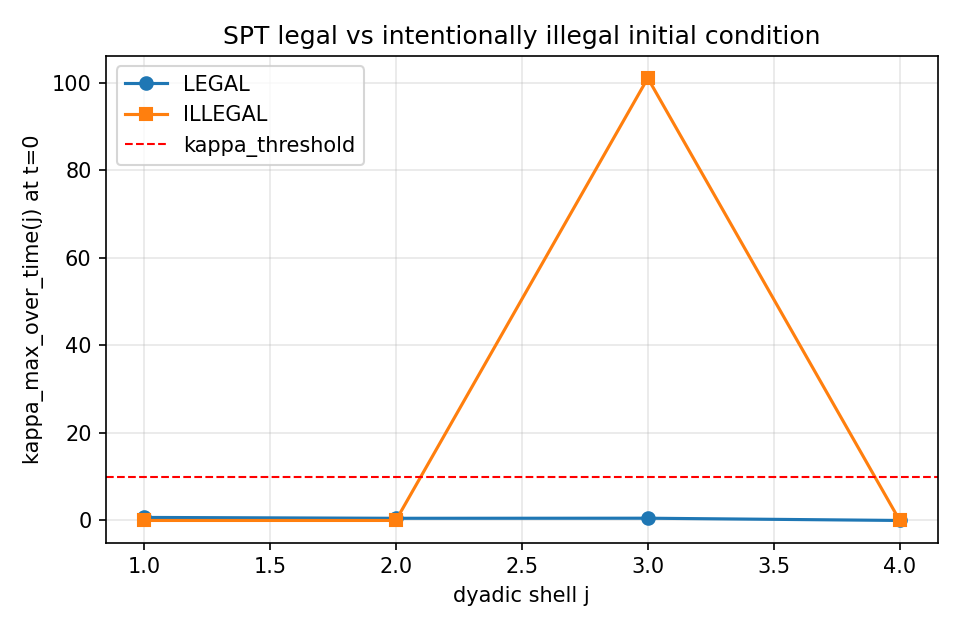
\includegraphics[width=0.92\linewidth]{../python/artifacts/paper/ns_spt_illegal_vs_legal.png}
  \caption{\textbf{LEGAL vs.\ ILLEGAL initial data under the same SBT-legality certificate.}
  The LEGAL baseline passes with $\max_j \kappa_j \approx O(1)$, while an intentionally localized
  shell ``wavepacket'' fails immediately with a very large concentration factor (e.g.\ $\max_j\kappa_j\sim 10^2$
  in the included demo). This illustrates that SBT-legality is a substantive restriction: it rules out
  strongly localized high-frequency initial conditions that trigger the wavepacket obstruction.}
  \label{fig:spt-illegal-vs-legal}
\end{figure}

\begin{remark}[What this does \emph{not} claim]
We do not prove that SBT-legality is preserved by Navier--Stokes evolution, nor that every smooth
initial datum is SBT-legal. The point is sharper: within this scaffold, \emph{bypassing the ICAP no-go}
requires an anti-localization/channelization hinge, and we can (i) state that hinge precisely,
(ii) mechanize the finite-dimensional inequality logic it relies on, and (iii) provide reproducible
diagnostics and certificates that test it on concrete initial conditions.
\end{remark}

\section{Experiments and reproducibility}
\label{sec:experiments}

This repository is organized so that every paper figure is generated by an explicit script,
with parameters and deterministic metadata recorded at runtime.
We emphasize again: the experiments in this section are \emph{diagnostics}, not proofs.
Their role is to (i) validate that the tooling is numerically consistent with the accounting-style
quantities we discuss, and (ii) provide empirical evidence for (or against) the proposed
SBT-legality / anti-localization hinge.

\subsection{Manifest-driven figure generation (single source of truth)}

The canonical list of paper artifacts is the manifest
\nolinkurl{paper/figures_manifest.json}.
Each manifest entry records:
(i) the producing script, (ii) a deterministic seed, (iii) the expected output paths for a
\texttt{.png} and a companion \texttt{.npz}, and (iv) stdout markers used as a lightweight check.

To generate \emph{all} figures (including slow ones) into \texttt{python/artifacts/paper/}, run:
\begin{verbatim}
python/scripts/ns_paper_figures.py --include-slow --clean
\end{verbatim}
To generate only the fast subset (intended for CI and quick checks), run:
\begin{verbatim}
python/scripts/ns_paper_figures.py --clean
\end{verbatim}

\subsection{Determinism and metadata}

Each figure script prints a JSON configuration line of the form:
\texttt{FIGURE\_CONFIG: \{...\}},
including the seed and simulation parameters (grid size, timestep, forcing parameters, thresholds).
Each figure also writes a companion \texttt{.npz} containing the plotted arrays and key scalars.
This enables two kinds of reproducibility:
\begin{itemize}
\item \textbf{Re-plot reproducibility:} the \texttt{.npz} contains all data needed to recreate the plot.
\item \textbf{Run determinism checks:} for the fast set, the generator supports
\texttt{--verify-determinism}, which re-runs the figure scripts and checks that the resulting
\texttt{.npz} hashes match.
\end{itemize}
In other words, the paper artifacts are treated like build products with a testable provenance chain.

\paragraph{Determinism scope.}
Our determinism checks verify byte-identical \texttt{.npz} outputs when rerunning in a fixed
software environment (same code, dependencies, and backend behavior). We do not claim bitwise
identity across arbitrary BLAS/FFT backends or thread schedules; for cross-platform reruns we
recommend pinning threads (e.g.\ \texttt{OMP\_NUM\_THREADS=1}, \texttt{MKL\_NUM\_THREADS=1})
and using tolerance-based numeric comparisons where appropriate.

\paragraph{Fast vs.\ slow figures.}
The manifest classifies figures as fast/slow/optional. Fast figures are intended for CI-style
checks, while slow figures are diagnostic enrichments and are not required for any mechanized claim.

\subsection{Main diagnostic figures (evidence, not proofs)}

We include a small set of representative figures in the main text.
The full index of paper artifacts (script $\leftrightarrow$ figure mapping) is maintained in
\texttt{docs/fluids/blowup/figures.md} and in the manifest.

\paragraph{Channel count (effective rank) by shell.}
This diagnostic estimates a minimal channel count $m_{95}$ capturing $95\%$ of shell variance
under a windowed PCA/SVD procedure. It is one empirical proxy for the ``finite channel'' premise
used in the anti-localization lemma template.

\paragraph{Interpreting pooled vs.\ windowed effective ranks.}
We report both windowed ranks (computed per time window) and pooled ranks (computed after pooling
snapshots across time and seeds). A pooled rank can exceed typical windowed ranks if the dominant
channel rotates over time: each window may be effectively one-dimensional, while the pooled dataset
spans a small subspace of dimension $>1$. We treat these as diagnostics of low-channel structure,
not as proof of a fixed global rank.

\begin{figure}[t]
  \centering
  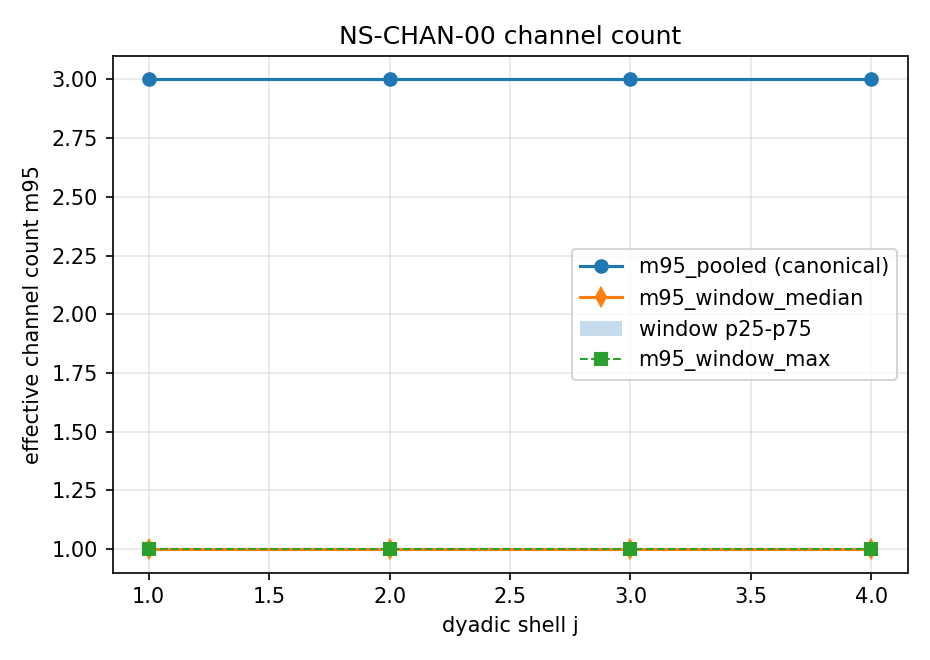
\includegraphics[width=0.92\linewidth]{../python/artifacts/paper/ns_channel_count.png}
  \caption{\textbf{Empirical channel count by shell.}
  We estimate an effective rank $m_{95}(j)$ capturing 95\% of variance from shell snapshots
  (pooled across seeds and windows; see script for details).
  This is diagnostic evidence relevant to finite-channel / sectorization narratives.}
  \label{fig:channel-count}
\end{figure}

\paragraph{Delocalization of learned channels.}
Given the channel decomposition used in Fig.~\ref{fig:channel-count}, we measure a delocalization proxy
for the extracted channel shapes and report an induced $\hat\eta_j$ consistent with
\eqref{eq:antiloc}--\eqref{eq:finite-channel-antiloc} (up to discretization and estimator choices).

\begin{figure}[t]
  \centering
  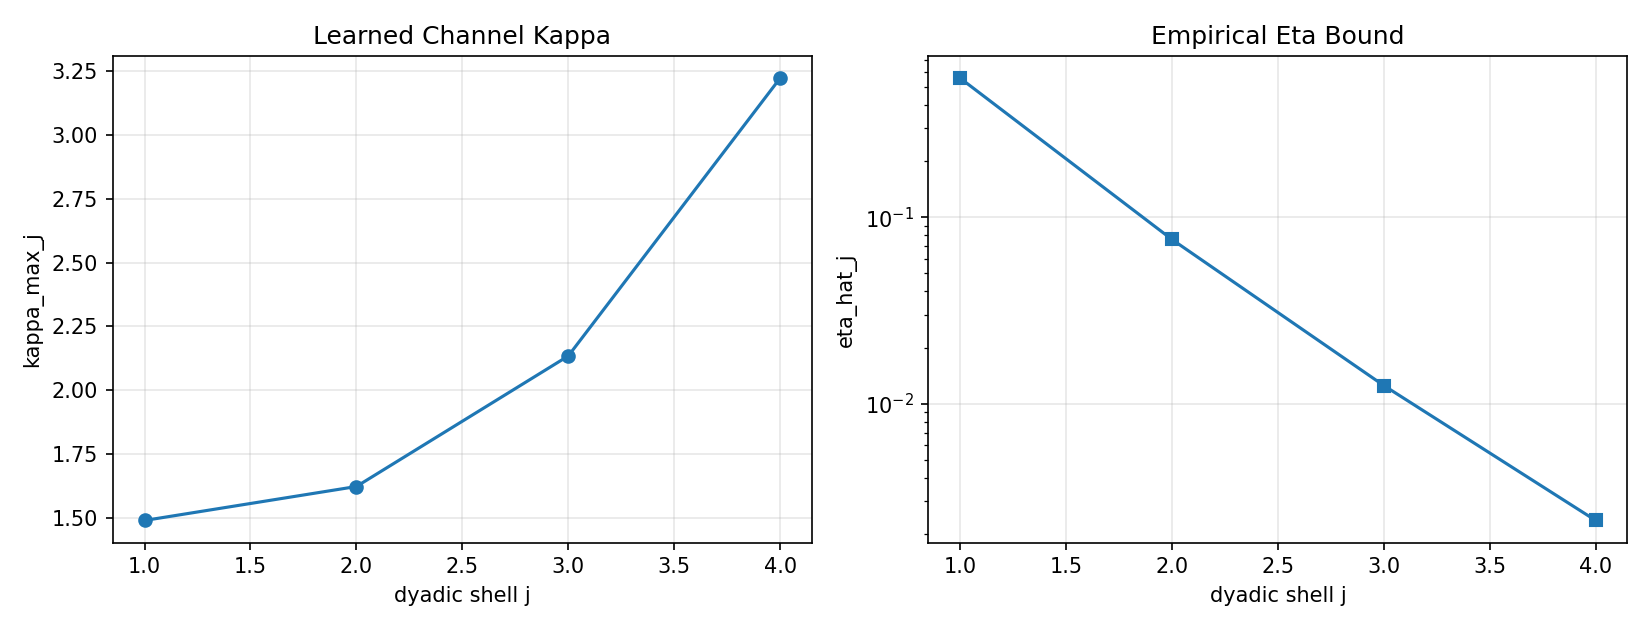
\includegraphics[width=0.92\linewidth]{../python/artifacts/paper/ns_channel_delocalization.png}
  \caption{\textbf{Empirical channel delocalization and induced anti-localization bound.}
  For each shell $j$, we evaluate a local mass functional on the learned channel shapes and report
  a worst-case delocalization proxy $\kappa$ and an induced $\hat\eta_j$.
  This is diagnostic-only evidence toward the anti-localization hinge.}
  \label{fig:channel-delocalization}
\end{figure}

\paragraph{Anti-localization sweep (SBT-legality evidence).}
We run a small sweep of short forced simulations and compute worst-case anti-localization metrics
over time windows (see Section~\ref{sec:spt-legal} for definitions). This is intended to answer:
``in tested regimes, do shell fields tend to avoid wavepacket-like localization?''

\begin{figure}[t]
  \centering
  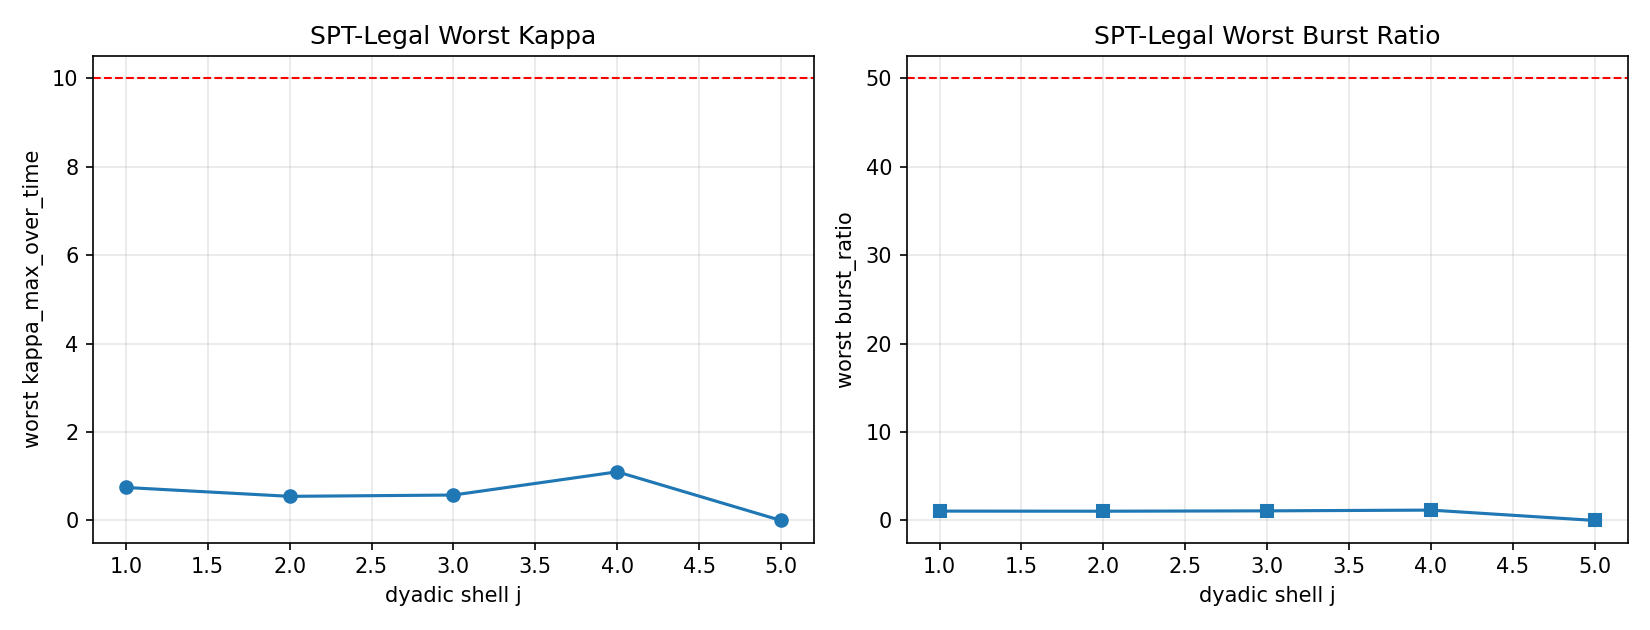
\includegraphics[width=0.92\linewidth]{../python/artifacts/paper/ns_spt_legal_sweep.png}
  \caption{\textbf{Anti-localization sweep (diagnostic).}
  Worst-case $\kappa_j$-style concentration factors over a small parameter/seed sweep.
  This supports plausibility of an anti-localization restriction in the tested window, but is not
  a worst-case theorem for Navier--Stokes.}
  \label{fig:spt-legal-sweep}
\end{figure}

\paragraph{LEGAL vs.\ ILLEGAL initial data (certificate nontriviality).}
Figure~\ref{fig:spt-illegal-vs-legal} (in Section~\ref{sec:spt-legal}) demonstrates that the
certificate is not vacuous: an intentionally localized shell construction fails immediately.

\paragraph{Toy Zeno gallery (intuition anchor).}
Finally, we include a purely mathematical toy gallery showing why the No-Zeno engine requires
both a work quantization and a divergence condition: with fast-growing capacity (or vanishing work),
Zeno can occur even when other bookkeeping looks benign.

\begin{figure}[t]
  \centering
  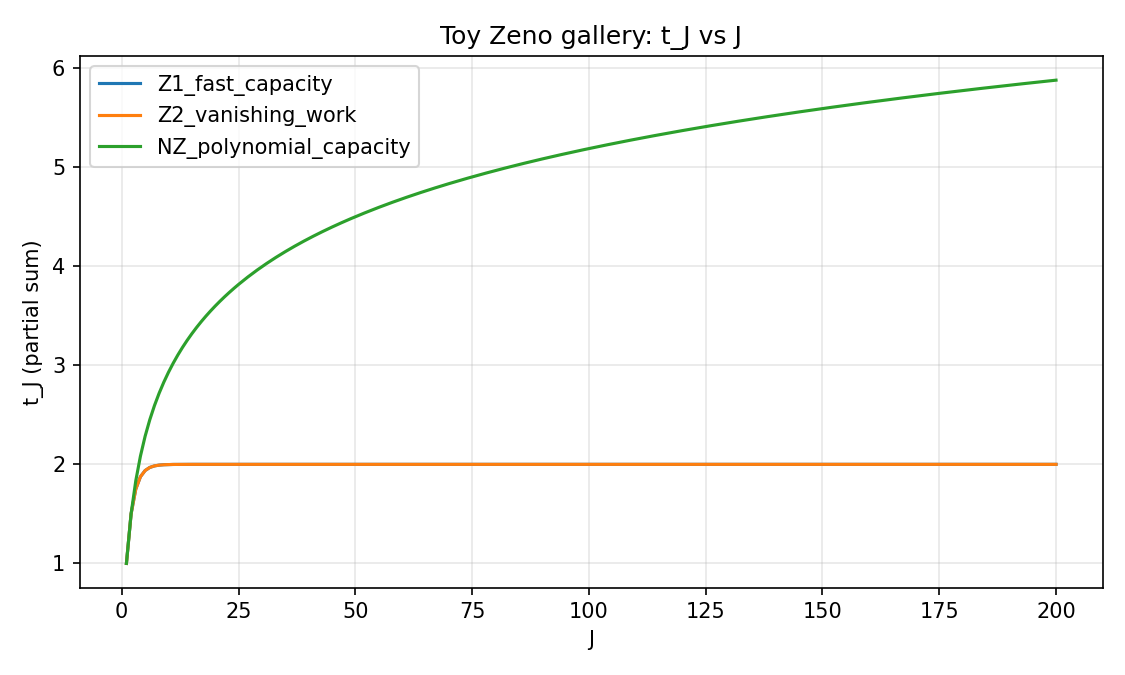
\includegraphics[width=0.92\linewidth]{../python/artifacts/paper/nsbu12_toy_zeno_gallery.png}
  \caption{\textbf{Toy Zeno gallery.}
  Three explicit sequences illustrate: (i) Zeno via fast-growing capacity (DIV fails),
  (ii) Zeno via vanishing work quantum (WORK fails), and (iii) a No-Zeno control with polynomial capacity.
  This figure is purely mathematical and serves as an intuition anchor for the mechanized No-Zeno logic.}
  \label{fig:toy-zeno}
\end{figure}

\section{Discussion, limitations, and what would be needed for Clay}\label{sec:discussion}

\paragraph{What this paper achieves.}
This repository and paper deliver a \emph{reproducible decision scaffold} for multiscale reasoning
in the style of the Six Birds framework.
We mechanize (in Lean) the core system-agnostic inequality logic behind a No-Zeno engine
(Section~\ref{sec:no-zeno-engine}), and we mechanize two additional abstract pillars:
(i) route-stability implies polynomial capacity growth (Section~\ref{sec:route-capacity}),
and (ii) a discrete no-go theorem showing that ICAP-style certificates imply pointwise
positive-gain bounds when the feasible input set contains localized tests
(Section~\ref{sec:no-go-icap}).
Separately, we provide a manifest-driven, deterministic Python pipeline that produces
all cited figures and their accompanying metadata (Section~\ref{sec:experiments}).

\paragraph{What this paper does \emph{not} claim.}
We do not prove the Clay 3D Navier--Stokes global regularity theorem.
All PDE-specific hinge claims that would be required for a Clay claim are stated explicitly
as OPEN assumptions elsewhere in the repository. Our emphasis is on (i) making the lemma chain
explicit and auditable, and (ii) showing precisely where and why the ``obvious'' ICAP/capacity
route collapses into a classical peak/strain channel unless one adds a genuine feasibility
restriction that excludes wavepacket-like localization.

\paragraph{Why the ICAP/capacity route does not automatically beat classical criteria.}
A uniform ICAP-style capacity certificate is an \emph{extremal} inequality: it bounds the maximal
positive work that the bridge can extract from \emph{all admissible inputs}.
The discrete no-go theorem (Section~\ref{sec:no-go-icap}) shows that if the feasible input set
is rich enough to contain basis-like localized tests, then any such ICAP bound immediately implies
a pointwise bound on the underlying positive-gain functional. In the PDE interpretation, the
corresponding gain bound aligns with a peak/strain channel (e.g.\ a supremum-type functional
controlling vortex stretching). This explains, structurally, why ``uniform ICAP solves Clay''
is not a free consequence of energy-based accounting.

\paragraph{What we do instead: an ``SBT-legal'' variant.}
Given the above obstruction, the only viable bypass within this scaffold is to restrict feasibility
so that localized wavepacket tests are \emph{not} admissible. We formalize this as an anti-localization
hinge and show that it can follow from finite-channel delocalized feasibility in a discrete model.
We then propose an operational certificate (computed by scripts in this repository) that checks
anti-localization-style metrics for initial data (Section~\ref{sec:spt-legal}).
This does not claim that legality is preserved under Navier--Stokes evolution; rather, it proposes
a concrete restricted theory where the No-Zeno engine becomes meaningful without smuggling in a
classical supremum regularity hypothesis.

\subsection{OPEN gaps: what would be needed for a Clay claim}
To turn this scaffold into a Clay regularity proof, one would need to establish PDE-facing statements
that go beyond what is currently proved here. Concretely:
\begin{itemize}
\item \textbf{A channelization theorem for the canonical NS packaged bridge:}
prove (or refute) that the feasible interface at shell $j$ is effectively low-channel and delocalized
in a sense strong enough to exclude wavepacket-like tests.
\item \textbf{Anti-localization as a theorem (not a certificate):}
prove that the actual NS-relevant feasible inputs satisfy an anti-localization inequality with
$\eta_j\to 0$ (or prove that intermittency produces counterexamples).
\item \textbf{A PDE bridge from ``No-Zeno'' to smooth continuation:}
show that the absence of a Zeno cascade (as defined by a canonical frontier) yields a continuation
criterion in an $H^s$ class, closing the loop from abstract increments to PDE regularity.
\end{itemize}

\subsection{Future work}
\paragraph{Theory (paper-facing).}
\begin{itemize}
\item Prove or refute a concrete Navier--Stokes statement implying wavepacket-exclusion for feasible inputs
(e.g.\ channelization/delocalization for a canonical packaged bridge object).
\item Clarify whether any such wavepacket-exclusion principle can be derived from NS structure without implicitly
assuming a classical peak-channel bound (BKM/Serrin-type) \citep{bkm_1984,serrin1962interior}.
\item Mechanize additional abstract ``interface calculus'' steps in Lean as they are used in the scaffold,
including alternative discrete feasibility models and their implications.
\end{itemize}

\paragraph{Numerics (repo-facing).}
\begin{itemize}
\item Push the existing diagnostic suite to higher $N$, longer horizons, and broader forcing/viscosity regimes,
and quantify robustness of channel and anti-localization metrics.
\item Stress-test intentionally illegal constructions (multiple localized patterns, multi-shell localization,
intermittency-like bursts) to map how the certificate fails.
\item Add sensitivity analyses: dependence of $\kappa_j$ and effective ranks on estimator choices (window sizes,
pooling strategy, basis choices).
\end{itemize}


\appendix
\clearpage
\section{Mechanized theorem index (Lean)}\label{app:theorem-index}

This appendix is the source of truth for what is mechanized in Lean.
All Lean results listed here are discrete (\(\mathbb{N}\)-indexed sums and finite-dimensional analogues), not continuum PDE formalizations.

\begin{table}[H]
\centering
\footnotesize
\renewcommand{\arraystretch}{1.15}
\setlength{\tabcolsep}{4pt}
\begin{tabular}{>{\raggedright\arraybackslash}p{0.18\linewidth}
                >{\raggedright\arraybackslash}p{0.22\linewidth}
                >{\raggedright\arraybackslash}p{0.18\linewidth}
                >{\raggedright\arraybackslash}p{0.30\linewidth}}
\toprule
\textbf{Paper statement} & \textbf{Lean theorem name} & \textbf{Lean file path} & \textbf{Hypotheses / conclusion (one line)} \\
\midrule
Section~\ref{sec:no-zeno-engine}, Theorem~\ref{thm:unbounded-sums-no-zeno}
& \nolinkurl{no_finite_upper_bound_of_increments_ge_of_sum_unbounded}
& \nolinkurl{formal/Fluids/Zeno.lean}
& If \(\Phi(n)\le t(n+1)-t(n)\) and partial sums of \(\Phi\) are unbounded, then \(t\) has no finite upper bound. \\

Section~\ref{sec:no-zeno-engine}, Theorem~\ref{thm:workcap-increment}
& \nolinkurl{workcap_div_le_increment}
& \nolinkurl{formal/Fluids/ZenoWorkCap.lean}
& From \(w(n)\le \mathrm{Cap}(n)\Delta t_n\) and \(\mathrm{Cap}(n)>0\), derive \(w(n)/\mathrm{Cap}(n)\le \Delta t_n\). \\

Section~\ref{sec:no-zeno-engine}, Theorem~\ref{thm:workcap-no-zeno}
& \nolinkurl{no_finite_upper_bound_of_workcap_of_sum_unbounded}
& \nolinkurl{formal/Fluids/ZenoWorkCap.lean}
& Combines work/cap division with unbounded partial sums of \(w/\mathrm{Cap}\) to conclude no finite upper bound on crossing times. \\

Section~\ref{sec:route-capacity}, Theorem~\ref{thm:route-capacity}
& \nolinkurl{route_capacity_poly_bound}; \nolinkurl{route_capacity_poly_bound_of_bounded_sum}
& \nolinkurl{formal/Fluids/RouteCapacity.lean}
& Recurrence \(C_{n+1}\le r_n C_n+e_n\), tame \(r_n\), and bounded mismatch sum imply polynomial bound \(C_n\lesssim (n+1)^p\). \\

Section~\ref{sec:route-capacity} (capacity aggregation step used in scaffold)
& \nolinkurl{max_sum_le_sum_max}; \nolinkurl{icap_sum_le_card_mul}
& \nolinkurl{formal/Fluids/ECTCap.lean}
& Moves \(\max(\cdot,0)\) through finite sums and bounds aggregated ICAP by sector count times per-atom bound. \\

Section~\ref{sec:spt-legal}, Lemma~\ref{lem:channel-antiloc}
& \nolinkurl{mass_cell_le_card_mul_deloc_mul_coeffEnergy}
& \nolinkurl{formal/Fluids/AntiLocalization.lean}
& In a finite-cell model (\texttt{Fintype}), \(m\) delocalized channels imply cell-mass bound \(\le m\kappa\mu(B)\sum_r a_r^2\). \\

Section~\ref{sec:no-go-icap}, Theorem~\ref{thm:icap-no-go}
& \nolinkurl{icap_implies_pointwise_pos_bound_of_basis_tests}
& \nolinkurl{formal/Fluids/IcapNoGo.lean}
& If ICAP holds for all inputs (including basis tests), then each pointwise positive gain is bounded by the ICAP constant. \\
\bottomrule
\end{tabular}
\end{table}

\clearpage
\section{Paper figure table (from the manifest)}\label{app:figure-table}

This appendix is generated from the single source of truth:
\nolinkurl{paper/figures_manifest.json}.
Do not edit the generated listing by hand.

% AUTO-GENERATED by python/scripts/ns_paper_appendix_figure_table.py
% Source: paper/figures_manifest.json
{\small\raggedright
\begin{description}
% id: fig_ns14_energy_ledger_3d
\item[\texttt{fig\_ns14\_energy\_ledger\_3d}] \textbf{class:} fast;
  \textbf{script:} \nolinkurl{python/scripts/ns14_energy_ledger_3d.py}\\
  \textbf{png:} \nolinkurl{python/artifacts/paper/ns14_energy_ledger_3d.png};
  \textbf{npz:} \nolinkurl{python/artifacts/paper/ns14_energy_ledger_3d_data.npz}.
% id: fig_ns15_uv_completion_3d
\item[\texttt{fig\_ns15\_uv\_completion\_3d}] \textbf{class:} fast;
  \textbf{script:} \nolinkurl{python/scripts/ns15_uv_completion_turns_on_3d.py}\\
  \textbf{png:} \nolinkurl{python/artifacts/paper/ns15_uv_completion_3d.png};
  \textbf{npz:} \nolinkurl{python/artifacts/paper/ns15_uv_completion_3d_data.npz}.
% id: fig_ns16_mu_convergence_3d
\item[\texttt{fig\_ns16\_mu\_convergence\_3d}] \textbf{class:} fast;
  \textbf{script:} \nolinkurl{python/scripts/ns16_mu_to_zero_convergence_3d.py}\\
  \textbf{png:} \nolinkurl{python/artifacts/paper/ns16_mu_convergence_3d.png};
  \textbf{npz:} \nolinkurl{python/artifacts/paper/ns16_mu_convergence_3d_data.npz}.
% id: fig_ns18_exponent_sanity
\item[\texttt{fig\_ns18\_exponent\_sanity}] \textbf{class:} fast;
  \textbf{script:} \nolinkurl{python/scripts/ns18_exponent_sanity_harness.py}\\
  \textbf{png:} \nolinkurl{python/artifacts/paper/ns18_exponent_sanity.png};
  \textbf{npz:} \nolinkurl{python/artifacts/paper/ns18_exponent_sanity_data.npz}.
% id: fig_nsbu12_toy_zeno_gallery
\item[\texttt{fig\_nsbu12\_toy\_zeno\_gallery}] \textbf{class:} fast;
  \textbf{script:} \nolinkurl{python/scripts/nsbu12_toy_zeno_gallery.py}\\
  \textbf{png:} \nolinkurl{python/artifacts/paper/nsbu12_toy_zeno_gallery.png};
  \textbf{npz:} \nolinkurl{python/artifacts/paper/nsbu12_toy_zeno_gallery_data.npz}.
% id: fig_ns_spt_illegal_vs_legal
\item[\texttt{fig\_ns\_spt\_illegal\_vs\_legal}] \textbf{class:} fast;
  \textbf{script:} \nolinkurl{python/scripts/ns_spt_illegal_ic_demo.py}\\
  \textbf{png:} \nolinkurl{python/artifacts/paper/ns_spt_illegal_vs_legal.png};
  \textbf{npz:} \nolinkurl{python/artifacts/paper/ns_spt_illegal_vs_legal_data.npz}.
% id: fig_nsbu21_route_capacity_numbers
\item[\texttt{fig\_nsbu21\_route\_capacity\_numbers}] \textbf{class:} slow;
  \textbf{script:} \nolinkurl{python/scripts/nsbu21_route_capacity_numbers.py}\\
  \textbf{png:} \nolinkurl{python/artifacts/paper/nsbu21_route_capacity_numbers.png};
  \textbf{npz:} \nolinkurl{python/artifacts/paper/nsbu21_route_capacity_numbers_data.npz}.
% id: fig_nsbu23_route_capacity_hypothesis_dense
\item[\texttt{fig\_nsbu23\_route\_capacity\_hypothesis\_dense}] \textbf{class:} slow;
  \textbf{script:} \nolinkurl{python/scripts/nsbu23_route_capacity_hypothesis_check.py}\\
  \textbf{png:} \nolinkurl{python/artifacts/paper/nsbu23_route_capacity_hypothesis_dense.png};
  \textbf{npz:} \nolinkurl{python/artifacts/paper/nsbu23_route_capacity_hypothesis_dense_data.npz}.
% id: fig_nsbu28_antilocalization
\item[\texttt{fig\_nsbu28\_antilocalization}] \textbf{class:} slow;
  \textbf{script:} \nolinkurl{python/scripts/nsbu28_antilocalization_diagnostic.py}\\
  \textbf{png:} \nolinkurl{python/artifacts/paper/nsbu28_antilocalization.png};
  \textbf{npz:} \nolinkurl{python/artifacts/paper/nsbu28_antilocalization_data.npz}.
% id: fig_nsbu29_antilocalization_sweep
\item[\texttt{fig\_nsbu29\_antilocalization\_sweep}] \textbf{class:} slow;
  \textbf{script:} \nolinkurl{python/scripts/nsbu29_antilocalization_sweep.py}\\
  \textbf{png:} \nolinkurl{python/artifacts/paper/nsbu29_antilocalization_sweep.png};
  \textbf{npz:} \nolinkurl{python/artifacts/paper/nsbu29_antilocalization_sweep_data.npz}.
% id: fig_ns_chan00_channel_count
\item[\texttt{fig\_ns\_chan00\_channel\_count}] \textbf{class:} slow;
  \textbf{script:} \nolinkurl{python/scripts/ns_chan00_channel_count.py}\\
  \textbf{png:} \nolinkurl{python/artifacts/paper/ns_channel_count.png};
  \textbf{npz:} \nolinkurl{python/artifacts/paper/ns_channel_count_data.npz}.
% id: fig_ns_chan01_channel_delocalization
\item[\texttt{fig\_ns\_chan01\_channel\_delocalization}] \textbf{class:} slow;
  \textbf{script:} \nolinkurl{python/scripts/ns_chan01_channel_delocalization.py}\\
  \textbf{png:} \nolinkurl{python/artifacts/paper/ns_channel_delocalization.png};
  \textbf{npz:} \nolinkurl{python/artifacts/paper/ns_channel_delocalization_data.npz}.
% id: fig_ns_spt_legal_sweep
\item[\texttt{fig\_ns\_spt\_legal\_sweep}] \textbf{class:} slow;
  \textbf{script:} \nolinkurl{python/scripts/ns_spt_legal_sweep.py}\\
  \textbf{png:} \nolinkurl{python/artifacts/paper/ns_spt_legal_sweep.png};
  \textbf{npz:} \nolinkurl{python/artifacts/paper/ns_spt_legal_sweep_data.npz}.
% id: fig_nsbu04_sgs_H
\item[\texttt{fig\_nsbu04\_sgs\_H}] \textbf{class:} optional;
  \textbf{script:} \nolinkurl{python/scripts/nsbu04_sgs_frequency_response.py}\\
  \textbf{png:} \nolinkurl{python/artifacts/paper/nsbu04_sgs_H.png};
  \textbf{npz:} \nolinkurl{python/artifacts/paper/nsbu04_sgs_H_data.npz}.
% id: fig_nsbu05_sgs_fit
\item[\texttt{fig\_nsbu05\_sgs\_fit}] \textbf{class:} optional;
  \textbf{script:} \nolinkurl{python/scripts/nsbu05_sgs_realization_fit.py}\\
  \textbf{png:} \nolinkurl{python/artifacts/paper/nsbu05_sgs_fit.png};
  \textbf{npz:} \nolinkurl{python/artifacts/paper/nsbu05_sgs_fit_data.npz}.
\end{description}
}


\section{How to run (commands and entry points)}\label{app:how-to-run}

All commands below are run from the repository root.

\subsection{Fast checks (CI-style)}
\begin{verbatim}
./check_python.sh
./check_lean.sh
\end{verbatim}

\subsection{Generate all paper figures from the manifest}
The manifest lives at \nolinkurl{paper/figures_manifest.json}.
To generate all figures (including slow ones) into \texttt{python/artifacts/paper/}:
\begin{verbatim}
python python/scripts/ns_paper_figures.py --include-slow --clean
\end{verbatim}
To also include optional figures:
{\small
\begin{verbatim}
python python/scripts/ns_paper_figures.py --include-slow --include-optional --clean
\end{verbatim}
}

\subsection{Determinism verification}
To re-run the manifest and verify deterministic metadata hashes for the fast set:
\begin{verbatim}
python python/scripts/ns_paper_figures.py --clean --verify-determinism
\end{verbatim}

\subsection{Build the paper PDF}
\begin{verbatim}
./check_paper.sh
\end{verbatim}
The paper sources live under \texttt{paper/}.

\section{Numerical method (minimal specification)}\label{app:numerics}

All Navier--Stokes experiments in this repository use a Fourier pseudo-spectral discretization \citep{canuto1988spectral} on
\(\T^3\) on an \(N\times N\times N\) grid. Fields are represented by Fourier coefficients \(\hat u(k)\),
and spatial derivatives are computed spectrally. Incompressibility is enforced by applying the
Leray projector in Fourier space, \(P(k)=I-\frac{k\otimes k}{|k|^2}\) for \(k\neq 0\) (and \(P(0)=I\)).

\paragraph{De-aliasing.}
Nonlinear terms are evaluated in physical space and transformed back to Fourier space.
To control aliasing, we apply a fixed de-aliasing mask corresponding to the \emph{2/3 rule} \citep{orszag1971aliasing}
(as implemented by \texttt{dealias\_mask\_3d} in the code). We report the resulting effective cutoff
\(k_{\mathrm{cut}}\) in the figure metadata, and use it when defining shell windows and
normalizations (e.g.\ in route-capacity diagnostics).

\paragraph{Time integration.}
We use a fixed time step \(\Delta t\) and advance the semi-discrete system using
\emph{an integrating-factor RK4 scheme} (\texttt{\_step\_ifrk4} in \texttt{ns3d\_spectral.py}).
The linear dissipative operator
\[
L(k)=-(\nu |k|^2 + \mu |k|^{2\alpha})
\]
is handled exactly through exponentials \(E=\exp(L\Delta t)\), \(E_{1/2}=\exp(L\Delta t/2)\),
while the nonlinear/forcing term is advanced with RK4 stages in the integrating-factor form.
All figures record \((N,\Delta t,t_{\max},\nu,\mu,\alpha)\) and forcing parameters in the printed
\texttt{FIGURE\_CONFIG} and stored \texttt{.npz} metadata.

\paragraph{Forcing.}
When forcing is enabled, scripts pass a deterministic Fourier-space forcing callback
\texttt{forcing\_hat\_fn}. In the paper diagnostics this is typically built from a seeded random field,
projected to divergence-free form, truncated to low wavenumbers \(|k|\le k_{\mathrm{force}}\),
de-aliased, and RMS-rescaled to the configured amplitude \texttt{forcing\_amp}. The forcing is
therefore deterministic given the script seed and configuration.

\paragraph{Scope.}
These simulations are used as \emph{diagnostics} for our multiscale certificates and hinge
metrics. We do not treat low-resolution runs as evidence about continuum blow-up or regularity,
and we explicitly separate mechanized algebraic claims (Lean) from numerical evidence (Python).


\bibliographystyle{plainnat}
\bibliography{refs}

\end{document}
